\begin{frame}{Sơ đồ Use Case - Quản trị viên}
\begin{figure}[H]
\centering
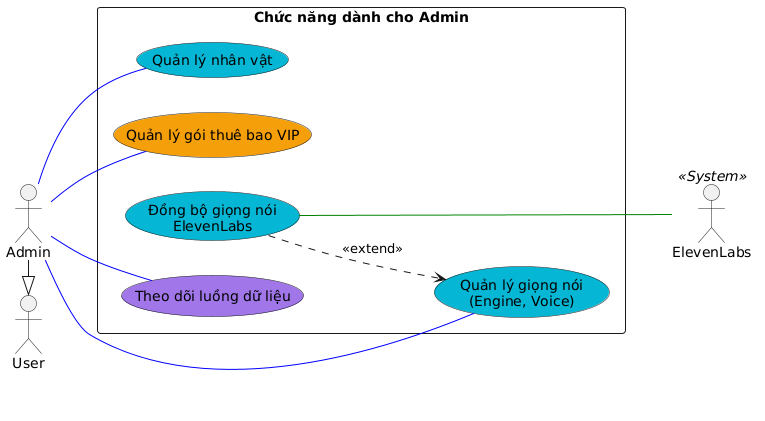
\includegraphics[width=\linewidth,height=0.72\textheight,keepaspectratio]{pictures/UML-UseCase-Admin.png}
\caption{Sơ đồ Use Case chức năng của quản trị viên}
\end{figure}

\note{
Sơ đồ Use Case dành cho quản trị viên (Admin).
Quản trị viên có các quyền hạn cao nhất trong hệ thống bao gồm: quản lý danh sách người dùng, quản lý cấu hình các gói thanh toán VIP, giám sát hệ thống, xem các báo cáo thống kê giao dịch và quản lý các tài liệu pháp luật chung trong CSDL tri thức của hệ thống.
}
\end{frame}
